\documentclass[11pt,a4paper]{article}

\usepackage[margin=2.2cm]{geometry}
\usepackage[T1]{fontenc}
\usepackage[utf8]{inputenc}
\usepackage{lmodern}
\usepackage{microtype}
\usepackage{amsmath,amssymb,mathtools,bm}
\usepackage{booktabs,tabularx,longtable,array,multirow}
\usepackage{graphicx}
\usepackage{caption,subcaption}
\usepackage{enumitem}
\usepackage{xcolor}
\usepackage{hyperref}
\usepackage{cleveref}
\usepackage{natbib}
\usepackage{tikz}
\usetikzlibrary{arrows.meta,positioning,fit,calc,shapes.geometric}
\usepackage{listings}
\usepackage{fancyhdr}
\usepackage{titlesec}
\usepackage{float}
\usepackage{siunitx}
\usepackage{url}
\usepackage[most]{tcolorbox}

\definecolor{deepblue}{RGB}{26,63,103}
\definecolor{softblue}{RGB}{231,240,249}
\definecolor{softgreen}{RGB}{233,245,238}
\definecolor{softorange}{RGB}{252,241,222}
\definecolor{softgray}{RGB}{244,245,247}
\definecolor{deepgreen}{RGB}{34,101,76}
\definecolor{deeporange}{RGB}{161,92,18}

\hypersetup{
  colorlinks=true,
  linkcolor=deepblue,
  citecolor=deepgreen,
  urlcolor=deeporange,
  pdftitle={Geometry-MMALS G1: From Audit Geometry to Grounded Functional Geometry},
  pdfauthor={Guillaume Harbonnier}
}

\pagestyle{fancy}
\fancyhf{}
\lhead{Geometry-MMALS G1}
\rhead{Research specification}
\cfoot{\thepage}
\setlength{\headheight}{14pt}

\titleformat{\section}{\Large\bfseries\color{deepblue}}{\thesection}{0.8em}{}
\titleformat{\subsection}{\large\bfseries\color{deepgreen}}{\thesubsection}{0.8em}{}
\titleformat{\subsubsection}{\normalsize\bfseries\color{deeporange}}{\thesubsubsection}{0.8em}{}

\setlist[itemize]{leftmargin=1.5em,itemsep=2pt,topsep=3pt}
\setlist[enumerate]{leftmargin=1.7em,itemsep=3pt,topsep=3pt}
\renewcommand{\arraystretch}{1.15}
\newcolumntype{Y}{>{\raggedright\arraybackslash}X}
\newcolumntype{C}{>{\centering\arraybackslash}X}

\newcommand{\MMALS}{\textsc{MMALS}}
\newcommand{\simplex}{\Delta^{H-1}}
\newcommand{\E}{\mathbb{E}}
\newcommand{\R}{\mathbb{R}}
\newcommand{\KL}{D_{\mathrm{KL}}}
\newcommand{\JS}{D_{\mathrm{JS}}}
\newcommand{\W}{\mathcal{W}_2}
\newcommand{\loss}{\mathcal{L}}
\newcommand{\norm}[1]{\left\lVert #1 \right\rVert}
\newcommand{\inner}[2]{\left\langle #1,#2 \right\rangle}

\newtcolorbox{plainbox}{
  colback=softblue,
  colframe=deepblue!35,
  boxrule=0.5pt,
  arc=2pt,
  left=8pt,right=8pt,top=7pt,bottom=7pt,
  before upper={\textbf{Plain-language reading.}~}
}

\newtcolorbox{claimbox}{
  colback=softgreen,
  colframe=deepgreen!40,
  boxrule=0.5pt,
  arc=2pt,
  left=8pt,right=8pt,top=7pt,bottom=7pt,
  before upper={\textbf{Admissible claim.}~}
}

\newtcolorbox{warningbox}{
  colback=softorange,
  colframe=deeporange!45,
  boxrule=0.5pt,
  arc=2pt,
  left=8pt,right=8pt,top=7pt,bottom=7pt,
  before upper={\textbf{Non-claim / falsification warning.}~}
}

\lstset{
  basicstyle=\ttfamily\small,
  backgroundcolor=\color{softgray},
  frame=single,
  rulecolor=\color{gray!35},
  breaklines=true,
  columns=fullflexible,
  showstringspaces=false,
  keywordstyle=\color{deepblue}\bfseries,
  commentstyle=\color{deepgreen}
}

\begin{document}

\begin{titlepage}
\centering
\vspace*{1.2cm}
{\Huge\bfseries\color{deepblue} Geometry-MMALS G1\par}
\vspace{0.3cm}
{\LARGE From Audit-Space Projections to Grounded Functional Geometry in Continual Learning\par}
\vspace{0.6cm}
{\large Conceptual, philosophical, mathematical, and experimental specification\par}
\vspace{1.2cm}
{\Large Guillaume Harbonnier\par}
\vspace{0.2cm}
{\normalsize Independent research program -- \href{https://github.com/gharbonnier78/geometry-mmalls-g1}{github.com/gharbonnier78/geometry-mmalls-g1}\par}
\vspace{0.8cm}
{\normalsize Version 1.0.1 -- June 2026\par}
\vfill
\begin{minipage}{0.88\textwidth}
\small
\textbf{Status.} This document is a research specification and implementation blueprint. It distinguishes validated or previously demonstrated MMALS mechanisms from proposed Geometry-MMALS hypotheses. It contains no claim that the G1 experiments have already succeeded, and it makes no claim of quantum advantage. Synthetic figures are explicitly labeled as illustrations. Version 1.0.1 is a release-audit patch: it clarifies the C0-only package status, adds pilot numeric gates, bridges TPUT and G1 notation, and labels the supervised G1-A geometric loss explicitly.
\end{minipage}
\vfill
\end{titlepage}

\begin{abstract}
Recent MMALS work introduced a useful geometry of audit and control traces: routes, hosts, memory, cost, stability, and objective vectors can be embedded in a structured decision space. That layer helps compare candidate policies and express goal-conditioned routing, but it does not yet establish that the learning system itself has discovered a meaningful geometry. This article specifies Geometry-MMALS G1, a grounded experimental program in which geometry is attributed only to internal representations, inferred contexts, routing distributions, host transformations, and their continual transport through learning time.

The proposal is deliberately staged. First, a frozen perceptual backbone isolates geometry already present in the sensory representation. Second, MMALS learns an inferred-context manifold, a route trajectory on the probability simplex, and host-specific transformation fields. Third, these structures are tested at four levels: descriptive order, predictive interpolation, causal intervention, and operational utility. A geometry is accepted only if it preserves known factors, predicts unseen contexts, responds coherently to controlled latent interventions, and improves concrete objectives such as accuracy, retention, cost, stability under drift, and host specialization. Host specialization is defined ecologically through contribution gain, ablation impact, representation separation, route-function stability, and cross-seed reproducibility rather than through raw selection frequency alone.

The primary protocol uses continuous RotatedMNIST because the rotation angle supplies an observable ground-truth factor. Secondary stages extend to Rotated FashionMNIST, Split-CIFAR10 with a mature frozen sensory grove, CORe50, and DomainNetMini. The mathematical specification includes Fisher-Rao geometry for routes, pull-back metrics for learned context coordinates, functional distances between hosts, graph and geodesic regularizers, optimal-transport alignment across continual-learning stages, and a dual memory model: reconstructive audit memory and synthetic compiled functional memory. Energy-guided routing is reserved for G2, and phase-aware or quantum-inspired routing for G3, only after G1 establishes real functional geometry.
\end{abstract}

\begin{plainbox}
The central question is not whether MMALS can draw attractive two-dimensional plots. It is whether neighboring real situations produce neighboring internal states; whether unseen intermediate situations can be handled by interpolation; whether moving an internal state in a measured direction causes the expected functional change; and whether this structure helps the system learn longer, forget less, route more efficiently, and specialize its hosts reproducibly.
\end{plainbox}

\tableofcontents
\newpage

\section{Motivation and scope}

\subsection{The distinction that motivates G1}

MMALS has recently used a structured vector of observable quantities---for example context confidence, route mass, host choice, memory state, cost, retention, stability, drift, and specialization indicators---to compare candidate traces and select policies under changing objectives. That construction is valuable. It is an \emph{external geometry of audit and control}: points are execution traces, coordinates are measurable indicators, and a controller selects among traces according to an objective.

However, the existence of this external geometry does not imply that the model has learned a geometrically meaningful internal organization. A scatterplot of audit variables can be useful even if the latent representation is collapsed, the router is discontinuous, the hosts are functionally redundant, or the apparent specialization is caused by an arbitrary index assignment. The G1 program therefore separates two objects:

\begin{align}
\text{External audit geometry} &: \quad a(x,t) \in \R^d,\\
\text{Internal functional geometry} &: \quad \Gamma(x,t)=\bigl(z_0,c,r,\{g_h(z_0)\}_{h=1}^H,z_M\bigr).
\end{align}

The first supports governance. The second must explain and improve learning.

\subsection{Problem statement}

The research problem is:

\begin{quote}
Can a continual-learning MMALS system learn an internal organization in which context proximity, routing transitions, host contributions, and memory transport form a coherent, predictive, causally testable, and operationally useful geometry?
\end{quote}

This question is narrower than a general claim that ``intelligence is geometry.'' It is also stronger than measuring Euclidean distances between arbitrary network parameters. Parameter coordinates are often non-identifiable: permutations, rescalings, and other symmetries may change weights while preserving behavior, so parameter-space distance need not correspond to functional distance \citep{dinh2017sharp}. G1 therefore prioritizes geometry of representations and functions.

\subsection{Concrete objectives}

The geometry is not an end in itself. It is intended to serve five MMALS objectives:

\begin{enumerate}[label=\textbf{G\arabic*.}]
\item \textbf{Accuracy}: choose transformations and routes that solve the current problem.
\item \textbf{Retention}: preserve useful route-function structures for earlier contexts.
\item \textbf{Cost}: avoid activating unnecessary hosts, transformations, and memory operations.
\item \textbf{Stability under drift}: detect and control structural change when inputs or tasks move.
\item \textbf{Host specialization}: produce a reproducible ecology of complementary functions rather than a single dominant host or arbitrary fragmentation.
\end{enumerate}

\begin{claimbox}
A successful G1 result would support the claim that geometry is an empirically grounded organizing principle for MMALS representations, routes, host functions, and memory transport. It would not yet support a claim of quantum computation, quantum advantage, consciousness, or universal intelligence.
\end{claimbox}

\section{Philosophical foundation}

The philosophical section is not decorative. It defines what counts as a meaningful geometric claim and prevents the research program from confusing metaphor, visualization, and mechanism.

\subsection{Structural rather than substance-first description}

The proposed stance is a pragmatic form of structural realism: MMALS knowledge is characterized primarily by stable relations among contexts, routes, transformations, memories, and outputs, not by the isolated identity of a parameter or unit \citep{worrall1989structural}. The claim is modest. It does not assert that all reality is mathematical structure. It says that the scientifically defensible content of a learned geometry lies in relational invariants that survive changes of seed, coordinate system, and representation basis.

A host therefore has no complete meaning in isolation. Its role is defined by:

\begin{itemize}
\item the contexts in which it is routed;
\item the transformation it contributes relative to alternative hosts;
\item the change in system performance when it is removed;
\item its compatibility with memory and with other hosts;
\item the stability of that role through time and across seeds.
\end{itemize}

This is consistent with MMALS's ecological metaphor, but the operational definitions are mathematical and testable.

\subsection{Process and transport rather than static storage}

Continual learning is inherently temporal. A static snapshot cannot distinguish healthy adaptation from destructive drift. G1 therefore treats learning as transport:

\begin{equation}
\mathcal{G}_1 \xrightarrow{T_{1\rightarrow2}} \mathcal{G}_2 \xrightarrow{T_{2\rightarrow3}} \cdots \xrightarrow{T_{T-1\rightarrow T}} \mathcal{G}_T,
\end{equation}

where \(\mathcal{G}_t\) denotes the internal route-function geometry after stage \(t\), and \(T_{t\rightarrow t+1}\) is the learned deformation or alignment between stages. Forgetting is not only a drop in accuracy; it may be a tearing of neighborhoods, a collapse of route diversity, a rotation of host functions, or a loss of recoverable correspondence.

\subsection{Operationalism: geometry must earn its name}

A geometric vocabulary is admitted only if it produces operational consequences. Four tests are required:

\begin{enumerate}
\item \textbf{Description}: known neighboring contexts are neighboring internally.
\item \textbf{Prediction}: unseen intermediate contexts can be inferred or interpolated.
\item \textbf{Intervention}: controlled movement along a latent direction changes behavior as predicted.
\item \textbf{Utility}: geometric constraints improve at least one target objective without unacceptable degradation of the others.
\end{enumerate}

The intervention requirement follows an interventionist view of causal explanation: a variable earns causal meaning when manipulating it changes the outcome in a stable, specific way \citep{woodward2003making}. Correlation between angle and a latent axis is suggestive; a tangent intervention with orthogonal controls is stronger.

\subsection{Ecological holism with decomposable evidence}

MMALS should not evaluate a host only by isolated accuracy. A host can be valuable because it stabilizes another host, preserves a route, reduces energy, or provides a transformation used rarely but critically. The architecture is therefore holistic at the system level but decomposable at the evidence level. Herbert Simon's notion of nearly decomposable systems is relevant: complex systems can have modules with strong internal organization and weaker, structured couplings among modules \citep{simon1962architecture}.

The practical implication is:

\begin{quote}
A host is specialized when its contribution is locally distinctive, causally useful, stable, and complementary within the complete MMALS ecosystem.
\end{quote}

\subsection{The simplicity axiom}

A well-designed MMALS system should remain as simple as the evidence allows. G1 therefore rejects premature use of curvature, topology, groupoids, quantum amplitudes, or exotic manifolds when Euclidean or simplex geometry is sufficient. Complexity is added only after a simpler null model fails.

The staged order is:

\begin{equation}
\boxed{\begin{gathered}\text{observed order} \rightarrow \text{predictive geometry} \rightarrow \text{causal geometry}\\\text{useful geometry} \rightarrow \text{energy} \rightarrow \text{phase-aware routing}\end{gathered}}
\end{equation}

\section{Conceptual architecture}

\subsection{Six internal objects and one external layer}

Geometry-MMALS G1 distinguishes the following objects.

\begin{table}[H]
\centering
\caption{Geometry-MMALS objects and their scientific roles.}
\label{tab:objects}
\begin{tabularx}{\textwidth}{@{}p{2.8cm}p{3.4cm}Y@{}}
\toprule
\textbf{Object} & \textbf{Symbol} & \textbf{Role} \\
\midrule
Sensory representation & \(z_0=P_\phi(x)\) & Frozen or slowly changing perceptual features. Establishes the geometry already present before MMALS. \\
Inferred context & \(c=q_\eta(z_0,m)\) & Low-dimensional or structured coordinate representing the current regime without task-id at inference. \\
Host transformation & \(z_h=g_{h,\theta_h}(z_0,c,m)\) & Functional transformation performed by host \(h\). \\
Route & \(r\in\Delta^{H-1}\) & Distribution of access to hosts; optionally sparse. \\
MMALS synthesis & \(z_M=A(r,z_1,\ldots,z_H)\) & Recombined representation used for prediction or control. \\
Memory state & \(m=(m^{\mathrm{rec}},m^{\mathrm{syn}})\) & Reconstructive audit memory plus synthetic/compiled functional memory. \\
Audit/control vector & \(a\in\R^d\) & External observability and objective-conditioned governance. Not itself proof of internal geometry. \\
\bottomrule
\end{tabularx}
\end{table}

\subsection{Architecture diagram}

\begin{figure}[H]
\centering
\resizebox{\textwidth}{!}{%
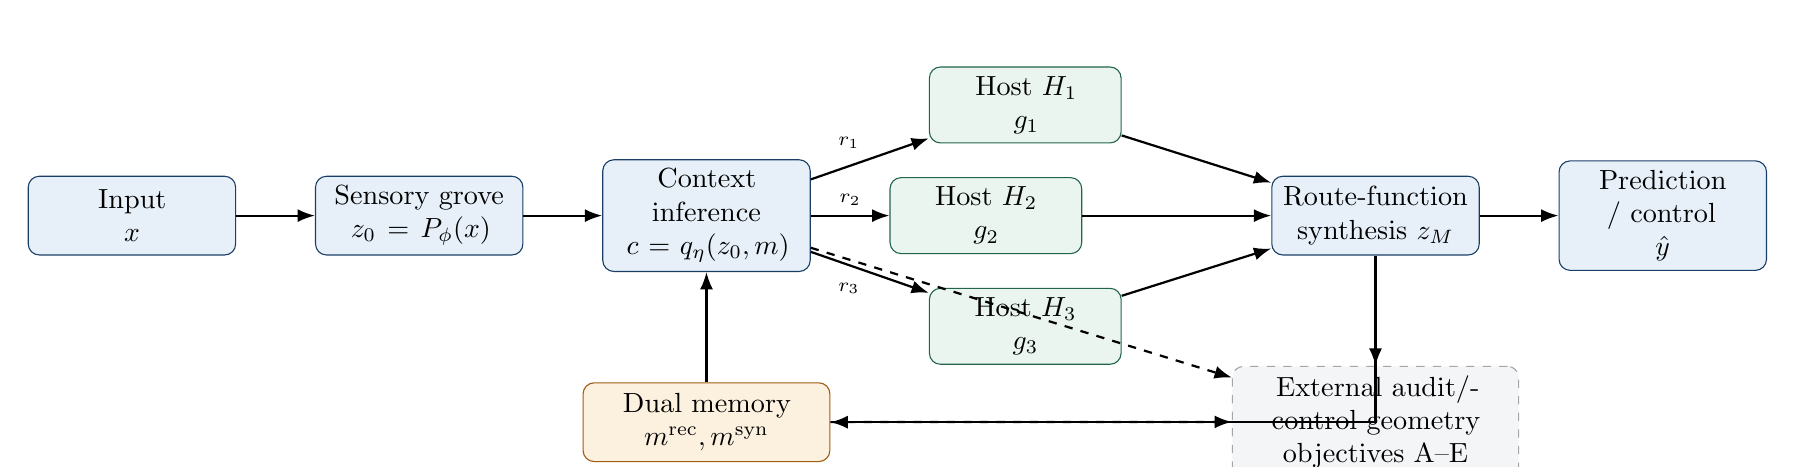
\begin{tikzpicture}[
  node distance=8mm and 10mm,
  box/.style={draw=deepblue,rounded corners,fill=softblue,minimum height=10mm,align=center,text width=24mm},
  host/.style={draw=deepgreen,rounded corners,fill=softgreen,minimum height=9mm,align=center,text width=22mm},
  mem/.style={draw=deeporange,rounded corners,fill=softorange,minimum height=10mm,align=center,text width=29mm},
  audit/.style={draw=gray!70,dashed,rounded corners,fill=softgray,minimum height=10mm,align=center,text width=34mm},
  arr/.style={-{Latex[length=2.2mm]},thick}
]
\node[box] (x) {Input\\\(x\)};
\node[box,right=of x] (p) {Sensory grove\\\(z_0=P_\phi(x)\)};
\node[box,right=of p] (c) {Context inference\\\(c=q_\eta(z_0,m)\)};
\node[host,above right=2mm and 15mm of c] (h1) {Host \(H_1\)\\\(g_1\)};
\node[host,right=of c] (h2) {Host \(H_2\)\\\(g_2\)};
\node[host,below right=2mm and 15mm of c] (h3) {Host \(H_3\)\\\(g_3\)};
\node[box,right=24mm of h2] (agg) {Route-function\\synthesis \(z_M\)};
\node[box,right=of agg] (y) {Prediction / control\\\(\hat y\)};
\node[mem,below=14mm of c] (mem) {Dual memory\\\(m^{\mathrm{rec}},m^{\mathrm{syn}}\)};
\node[audit,below=14mm of agg] (audit) {External audit/control geometry\\objectives A--E};

\draw[arr] (x)--(p);
\draw[arr] (p)--(c);
\draw[arr] (c)--node[above left,font=\scriptsize]{\(r_1\)}(h1);
\draw[arr] (c)--node[above,font=\scriptsize]{\(r_2\)}(h2);
\draw[arr] (c)--node[below left,font=\scriptsize]{\(r_3\)}(h3);
\draw[arr] (h1)--(agg);
\draw[arr] (h2)--(agg);
\draw[arr] (h3)--(agg);
\draw[arr] (agg)--(y);
\draw[arr] (mem)--(c);
\draw[arr] (agg)|-(mem);
\draw[arr,dashed] (c)--(audit);
\draw[arr,dashed] (agg)--(audit);
\draw[arr,dashed] (mem)--(audit);
\end{tikzpicture}%
}
\caption{Conceptual Geometry-MMALS G1 architecture. Geometry is investigated inside the perceptual, context, route, host, synthesis, and memory layers. The audit/control geometry remains a separate governance layer.}
\label{fig:architecture}
\end{figure}

\subsection{The mature sensory grove as an explicit host boundary}

The sensory extractor is not automatically a MMALS host. G1 begins with a frozen encoder \(P_\phi\) to separate two hypotheses:

\begin{description}
\item[Perceptual geometry hypothesis.] The backbone already organizes images by class, pose, or rotation.
\item[MMALS geometry hypothesis.] The context router and hosts add a functionally useful organization beyond the backbone.
\end{description}

Later experiments may promote the sensory grove to a functional host if it participates in routing, has an ablation-defined contribution, and adapts under explicit memory constraints. In G1, freezing it is a methodological control.

\section{Mathematical specification}

\subsection{Data, context factor, and continual stream}

Let \(x\in\mathcal{X}\) be an input and \(y\in\mathcal{Y}\) its target. A grounded context factor \(u\in\mathcal{U}\) generates or indexes a transformation of the observation. In the first experiment, \(u=\theta\) is the image rotation angle. The data distribution is

\begin{equation}
(x,y)\sim p_t(x,y\mid u), \qquad u\sim \pi_t(u),
\end{equation}

where the index \(t\) denotes a continual-learning stage. The model does not receive a task identifier at inference. The factor \(u\) is retained by the evaluator as ground truth.

\subsection{Perceptual representation}

A sensory encoder maps the input to a representation:

\begin{equation}
 z_0=P_\phi(x)\in\R^{d_0}.
\end{equation}

In the primary G1 experiment, \(\phi\) is trained once on a declared reference protocol and then frozen. This avoids attributing every geometric pattern to the router.

\subsection{Context manifold}

The inferred context is

\begin{equation}
 c=q_\eta(z_0,m)\in\mathcal{M}_C,
\end{equation}

where \(\mathcal{M}_C\) may initially be Euclidean. If \(q_\eta\) is differentiable, a local pull-back metric can be defined from a decoder or task map \(F\):

\begin{equation}
 G_C(c)=J_F(c)^\top J_F(c)+\epsilon I.
\end{equation}

The intrinsic length of a path \(\gamma:[0,1]\rightarrow\mathcal{M}_C\) is

\begin{equation}
 L(\gamma)=\int_0^1 \sqrt{\dot\gamma(s)^\top G_C(\gamma(s))\dot\gamma(s)}\,ds.
\end{equation}

This follows standard pull-back geometry used to study learned latent spaces \citep{arvanitidis2018latent,shao2018riemannian}. G1 does not assume curvature is necessary; the Euclidean metric is the first null model.

\subsection{Route geometry on the simplex}

The router outputs

\begin{equation}
 r=R_\psi(z_0,c,m,g)\in\simplex,
 \qquad r_h\ge0,\quad \sum_{h=1}^H r_h=1,
\end{equation}

where \(g\) is an optional objective vector. Routing distributions live on a probability simplex, for which Euclidean distance is often a poor default near boundaries. G1 therefore reports multiple metrics, including Jensen-Shannon divergence and the Fisher-Rao/Hellinger geodesic:

\begin{align}
 d_{\mathrm{JS}}(r,r') &= \sqrt{\JS(r\|r')},\\
 d_{\mathrm{FR}}(r,r') &= 2\arccos\left(\sum_{h=1}^H\sqrt{r_hr'_h}\right).
\end{align}

The square-root map \(r\mapsto 2(\sqrt{r_1},\ldots,\sqrt{r_H})\) embeds the simplex in a sphere and makes route interpolation geometrically interpretable.

\subsection{Host transformations and synthesis}

Each host computes

\begin{equation}
 z_h=g_{h,\theta_h}(z_0,c,m)\in\R^{d_M}.
\end{equation}

The synthesis operator is initially a weighted sum with optional normalization:

\begin{equation}
 z_M=\sum_{h=1}^H r_h z_h,
 \qquad \hat y=D_\omega(z_M).
\end{equation}

The route-function object is not merely \(r\). It is

\begin{equation}
 \Gamma(x)=\left(r(x),\;\{g_h(z_0(x),c(x),m)\}_{h=1}^H,\;z_M(x)\right).
\end{equation}

Two examples may have similar routes but different host outputs, or similar outputs through different routes. Both distinctions must be audited.

\subsection{Functional distance between hosts}

Parameter distance between hosts is insufficient because permuted or rescaled parameters can implement similar functions. Define a probe distribution \(\nu\) and a functional distance

\begin{equation}
 d_F(h,k)^2=\E_{x\sim\nu}\left[\norm{g_h(z_0(x),c(x),m)-g_k(z_0(x),c(x),m)}_2^2\right].
\end{equation}

A task-aware variant measures predictive disagreement:

\begin{equation}
 d_{\mathrm{pred}}(h,k)=\E_{x\sim\nu}\left[\JS\bigl(p_h(\cdot\mid x)\,\|\,p_k(\cdot\mid x)\bigr)\right].
\end{equation}

Representation similarity is also assessed with linear CKA \citep{kornblith2019cka}; topological divergence can be added as a higher-order diagnostic rather than a primary gate \citep{barannikov2022rtd}.

\subsection{Grounded geometric correspondence}

Let \(d_U(u_i,u_j)\) be the known distance between context factors; for rotation,

\begin{equation}
 d_U(\theta_i,\theta_j)=\min\bigl(|\theta_i-\theta_j|,360^\circ-|\theta_i-\theta_j|\bigr).
\end{equation}

The learned distances are

\begin{align}
 d_C(i,j)&=d_{\mathcal{M}_C}(c_i,c_j),\\
 d_R(i,j)&=d_{\mathrm{FR}}(r_i,r_j),\\
 d_M(i,j)&=\norm{z_{M,i}-z_{M,j}}_2.
\end{align}

A first descriptive criterion is rank agreement:

\begin{equation}
 \rho_C=\operatorname{Spearman}\bigl(d_U,d_C\bigr),\qquad
 \rho_R=\operatorname{Spearman}\bigl(d_U,d_R\bigr).
\end{equation}

A stronger local-isometry criterion uses normalized stress \citep{kruskal1964mds}:

\begin{equation}
 \operatorname{Stress}(D_U,D_C)=
 \sqrt{\frac{\sum_{i<j}(\tilde d_U(i,j)-\tilde d_C(i,j))^2}{\sum_{i<j}\tilde d_U(i,j)^2}}.
\end{equation}

\subsection{Geometric regularizers}

For pairs of examples \((i,j)\), define a neighborhood weight

\begin{equation}
 w_{ij}=\exp\left(-\frac{d_U(u_i,u_j)^2}{2\sigma_U^2}\right).
\end{equation}

The route smoothness loss is

\begin{equation}
 \loss_{\mathrm{route\text{-}geo}}=
 \frac{1}{|\mathcal{P}|}\sum_{(i,j)\in\mathcal{P}}w_{ij}\,d_{\mathrm{FR}}(r_i,r_j)^2.
\end{equation}

To avoid trivial constant routes, add a contrastive margin for distant contexts:

\begin{equation}
 \loss_{\mathrm{far}}=
 \frac{1}{|\mathcal{N}|}\sum_{(i,j)\in\mathcal{N}}
 \max\bigl(0,\mu-d_{\mathrm{FR}}(r_i,r_j)\bigr)^2.
\end{equation}

A distance-matching loss directly aligns route and factor geometry:

\begin{equation}
 \loss_{\mathrm{stress}}=\frac{1}{|\mathcal{B}|^2}\sum_{i<j}
 \left(\frac{d_R(i,j)}{\bar d_R+\epsilon}-\frac{d_U(i,j)}{\bar d_U+\epsilon}\right)^2.
\end{equation}

In later tasks where \(u\) is unknown, pseudo-neighborhoods are constructed from augmentations, temporal continuity, prototype confidence, or verified memory anchors. Ground-truth geometry is used only in the controlled G1 benchmark. The notebook implementation is therefore labeled \emph{G1-A supervised/grounded}: the true rotation angle shapes a declared geometry loss during training but is never passed to the deployable router at inference time. Any variant claiming geometry discovery without supervision must remove this term and report the comparison separately.

\subsection{Host specialization as an ecological property}

Raw route dominance is not specialization. G1 combines five evidence families.

\subsubsection{Route selectivity}

For host \(h\), let \(\bar r_h(u)=\E[r_h\mid u]\). Route entropy is

\begin{equation}
 H(r)=-\sum_h r_h\log(r_h+\epsilon),
\end{equation}

and context selectivity can be measured by mutual information \(I(H;U)\) after sampling a host from \(r\). High mutual information alone is insufficient because a brittle hard partition can score highly.

\subsubsection{Contribution gain}

Let \(\ell\) be the evaluation loss. Remove or neutralize host \(h\) and renormalize the route. The local contribution is

\begin{equation}
 \Delta_h(u)=\E[\ell(\hat y_{-h},y)-\ell(\hat y,y)\mid u].
\end{equation}

Positive \(\Delta_h(u)\) means the host contributes useful function in region \(u\). A specialization map is the vector \(\bm\Delta_h=(\Delta_h(u_1),\ldots,\Delta_h(u_K))\).

\subsubsection{Representation separation}

Hosts should not all produce the same feature map. Pairwise CKA, predictive disagreement, and functional distance quantify redundancy. Excessive separation is also undesirable if it fragments the problem and destroys transfer. G1 therefore seeks \emph{structured complementarity}, not maximum diversity.

\subsubsection{Route-function stability}

For an anchor set \(A_u\) retained across stages,

\begin{equation}
 S^{(h)}_{\mathrm{RF}}(t,t+1)=1-
 \frac{\E_{x\in A_u}\norm{g_{h,t+1}(x)-Q_hg_{h,t}(x)}}{Z_h},
\end{equation}

where \(Q_h\) is an orthogonal alignment and \(Z_h\) normalizes scale. Route stability uses \(d_{\mathrm{FR}}\). A stable host is not necessarily frozen; it may adapt while preserving its local function.

\subsubsection{Cross-seed reproducibility}

Host indices are exchangeable. Hosts are matched across seeds with the Hungarian algorithm using a cost based on contribution-map distance, CKA, and route-profile distance. Specialization is credible only when matched roles recur across seeds.

\subsection{Dual memory geometry}

MMALS distinguishes two complementary memories.

\paragraph{Reconstructive audit memory.}
Stores enough information to replay or reconstruct the route-function path:

\begin{equation}
 m^{\mathrm{rec}}=\{u,\;c,\;r,\;\text{host IDs},\;\text{transform summaries},\;\hat y,\;\text{evidence}\}.
\end{equation}

Its purpose is audit, debugging, reproducibility, and causal comparison.

\paragraph{Synthetic compiled functional memory.}
Compresses repeated route-function patterns into prototypes, adapters, basis functions, or cached transformations:

\begin{equation}
 m^{\mathrm{syn}}=\{\pi_k,\bar c_k,\bar r_k,\bar T_k,\Sigma_k\}_{k=1}^K.
\end{equation}

Its purpose is cheap reuse. The two memories must remain linked: a compiled synthesis should retain pointers or checksums sufficient to recover its evidence lineage.

\subsection{Continual transport and geometric drift}

At stage \(t\), let \(Z_t^u\) be the matrix of anchor representations for context region \(u\). Because representation coordinates may rotate, compare aligned states:

\begin{equation}
 Q_t^u=\arg\min_{Q^\top Q=I}\norm{Z_{t+1}^u-Z_t^uQ}_F^2.
\end{equation}

The aligned representation drift is

\begin{equation}
 D_Z^u(t,t+1)=\frac{\norm{Z_{t+1}^u-Z_t^uQ_t^u}_F}{\norm{Z_t^u}_F+\epsilon}.
\end{equation}

Distributional transport can be measured with entropic optimal transport \citep{cuturi2013sinkhorn,peyre2019ot}:

\begin{equation}
 D_{\mathrm{OT}}^u(t,t+1)=\W\bigl(\mu_t^u,\mu_{t+1}^u\bigr).
\end{equation}

The full route-function drift is

\begin{equation}
 D_{\Gamma}^u=\lambda_ZD_Z^u+\lambda_R\E[d_{\mathrm{FR}}(r_t,r_{t+1})]
+\lambda_F\E[d_F(g_t,g_{t+1})].
\end{equation}

Representational drift is not automatically forgetting; a network may drift while retaining performance \citep{pashakhanloo2023drift}. G1 therefore reports both drift and functional retention.

\subsection{Carbon cost and phosphorus gain}

The original MMALS ecological language is retained as a controlled metaphor.

\paragraph{Carbon cost.}
Represents diffusion and transformation cost, not literal carbon emissions:

\begin{equation}
 C_{\mathrm{carbon}}=
 \alpha_H H(r)+\alpha_A\sum_h\mathbb{1}[r_h>\tau]
 +\alpha_F\sum_h r_h\,\mathrm{FLOPs}(g_h)
 +\alpha_M C(m).
\end{equation}

\paragraph{Phosphorus gain.}
Represents functional contribution, primarily measured by ablation:

\begin{equation}
 G_{\mathrm{phosphorus}}=\sum_h r_h\,[\Delta_h(u)]_+.
\end{equation}

A route is ecologically efficient when it purchases defensible functional gain at low cost.

\subsection{Multiobjective training and control}

Let the goal vector be

\begin{equation}
 g=(w_A,w_B,w_C,w_D,w_E)\in\Delta^4,
\end{equation}

for accuracy, retention, cost, drift stability, and specialization. A generic objective is

\begin{equation}
\begin{split}
\loss_{\mathrm{total}}(g)=
&w_A\loss_{\mathrm{task}}
+w_B\loss_{\mathrm{ret}}
+w_C C_{\mathrm{carbon}}
+w_D\loss_{\mathrm{transport}}\\
&+w_E\loss_{\mathrm{specialization}}
+\lambda_{\mathrm{geo}}\loss_{\mathrm{geometry}}.
\end{split}
\end{equation}

G1 does not require joint training over all goals. The first implementation can export trace candidates and apply goal vectors post hoc. The critical test is whether routing changes in a rational and reproducible way when the goal changes, while future-retention constraints are respected.

\section{What counts as real Geometry-MMALS evidence?}

\subsection{A four-level proof ladder}

\begin{table}[H]
\centering
\caption{The G1 proof ladder. Each level includes the previous one.}
\label{tab:proof}
\begin{tabularx}{\textwidth}{@{}p{1.2cm}p{3.2cm}Y Y@{}}
\toprule
\textbf{Level} & \textbf{Name} & \textbf{Required evidence} & \textbf{What it excludes} \\
\midrule
L1 & Descriptive geometry & Known context distances correlate with latent and route distances; neighborhoods and order are preserved beyond null models. & Arbitrary clusters and purely decorative projections. \\
L2 & Predictive geometry & Unseen intermediate contexts are located and routed better than nearest-task or categorical baselines. & Memorization of discrete training contexts. \\
L3 & Causal geometry & Tangent interventions cause predicted route/function changes; orthogonal and random directions do not. & Passive correlation without mechanism. \\
L4 & Operational geometry & Geometric constraints improve interpolation, retention, stability, cost, or specialization under matched budgets. & Geometry that is measurable but useless. \\
\bottomrule
\end{tabularx}
\end{table}

\subsection{Why PCA and UMAP are not proof}

PCA, UMAP, and t-SNE are useful visual diagnostics, but any two-dimensional projection can distort distances, invent apparent clusters, or hide overlap. Manifold-learning methods such as Isomap and LLE explicitly seek low-dimensional structure \citep{tenenbaum2000isomap,roweis2000lle}, but their plots remain hypotheses. G1 uses quantitative distances, held-out prediction, interventions, and matched controls as primary evidence.

\subsection{Null models}

Every geometric claim is compared with at least four nulls:

\begin{enumerate}
\item shuffled context labels \(u\);
\item random orthogonal projections of equal dimension;
\item an untrained router with matched output entropy;
\item a backbone-only model with no MMALS transformation.
\end{enumerate}

Additional nulls include route permutations, host-index permutations, random latent directions, and equal-capacity dense networks.

\section{Primary experiment: continuous RotatedMNIST}

\subsection{Why rotation is the correct first test}

RotatedMNIST is not chosen because it is a difficult final benchmark. It is chosen because it supplies a known, continuous factor with a simple topology. The evaluator knows the angle; the model must infer it from the image. This lets us ask whether the learned geometry respects a real transformation rather than an arbitrary task label.

\subsection{Data protocol}

A recommended first schedule is:

\begin{align}
\Theta_{\mathrm{train}}&=\{-60^\circ,-30^\circ,0^\circ,30^\circ,60^\circ\},\\
\Theta_{\mathrm{interp}}&=\{-45^\circ,-15^\circ,15^\circ,45^\circ\},\\
\Theta_{\mathrm{extra}}&=\{-75^\circ,75^\circ\}.
\end{align}

Training can be either stage-wise or streaming. The primary claim uses stage-wise continual learning because it exposes retention and transport. A secondary boundary-free stream samples slowly varying angles with occasional jumps.

\subsection{Compared systems}

\begin{table}[H]
\centering
\caption{Minimum comparison set. Hyperparameters are selected on validation data, never on final test performance.}
\label{tab:systems}
\begin{tabularx}{\textwidth}{@{}p{3.2cm}Y p{3.4cm}@{}}
\toprule
\textbf{System} & \textbf{Purpose} & \textbf{Budget rule} \\
\midrule
Frozen encoder + linear head & Measures geometry and performance already available in the sensory grove. & Same encoder and evaluation data. \\
Dense shared network & Tests whether MMALS routing is necessary. & Matched active parameters and FLOPs. \\
Sparse MoE router & Standard conditional-computation baseline \citep{shazeer2017moe,fedus2022switch}. & Matched hosts, top-\(k\), active compute. \\
MMALS softmax & Current non-geometric routing baseline. & Same architecture as G1 geometry model. \\
MMALS + route geometry & Adds simplex smoothness and stress losses. & Same parameters; training overhead reported. \\
MMALS + full G1 & Adds specialization and transport constraints. & Same host count and memory budget. \\
EWC, replay, GEM & Continual-learning controls \citep{kirkpatrick2017ewc,lopezpaz2017gem,rolnick2019replay}. & Validation-selected sweeps; memory matched where relevant. \\
Joint upper bound & Trains on all stages jointly; not deployable as CL. & Same architecture, all data access. \\
\bottomrule
\end{tabularx}
\end{table}

Baseline hardening is mandatory: EWC coefficient, replay size, learning rate, sparsity, host count, and router temperature are swept on validation streams. Weak arbitrary defaults would invalidate the comparison.

\subsection{Training sequence}

\begin{enumerate}
\item Pretrain the sensory encoder on the declared reference set; freeze it.
\item Initialize context inference, hosts, router, synthesis, and classifier.
\item Train stage \(t\) on angle \(\theta_t\) without task-id at inference.
\item After every epoch, evaluate all previous, current, interpolation, and extrapolation angles.
\item Store anchor examples or feature prototypes according to the memory budget.
\item Export route-function traces for every evaluation point.
\item Repeat for 5--10 seeds; 10 seeds are preferred for the final claim.
\end{enumerate}

\subsection{Descriptive tests}

For each representation layer \(z_0,c,r,z_h,z_M\), measure:

\begin{itemize}
\item Spearman correlation between angular distance and representation distance;
\item neighborhood preservation at \(k\in\{5,10,20\}\);
\item normalized stress;
\item intrinsic dimension estimates;
\item CKA across stages and seeds;
\item route entropy and host occupancy;
\item topology divergence as an exploratory diagnostic.
\end{itemize}

The backbone-vs-MMALS delta is essential:

\begin{equation}
 \Delta\rho=\rho(z_M)-\rho(z_0).
\end{equation}

A positive \(\Delta\rho\) suggests that MMALS adds organization; a negative value may still be acceptable if predictive or operational results improve, but the trade-off must be explained.

\subsection{Predictive interpolation tests}

For an unseen angle \(\theta^*\) between two trained angles \(\theta_a<\theta^*<\theta_b\), compare the observed route with a geodesic interpolation:

\begin{equation}
 \hat r(\theta^*)=\operatorname{GeoInterp}_{\Delta}
 \left(r(\theta_a),r(\theta_b);\lambda\right),
 \quad \lambda=\frac{\theta^*-\theta_a}{\theta_b-\theta_a}.
\end{equation}

The interpolation error is

\begin{equation}
 E_{\mathrm{interp}}=d_{\mathrm{FR}}\left(r(\theta^*),\hat r(\theta^*)\right).
\end{equation}

The functional test compares accuracy and calibration against:

\begin{itemize}
\item nearest trained angle;
\item linear interpolation in logits;
\item unconstrained softmax MMALS;
\item oracle-angle routing, reported only as an upper diagnostic bound.
\end{itemize}

\subsection{Causal tangent intervention}

Estimate an angle tangent in context space using local regression:

\begin{equation}
 v_\theta(c)=\arg\min_v\sum_{j\in\mathcal{N}(c)}
 \left((\theta_j-\theta_c)-v^\top(c_j-c)\right)^2+\lambda\norm v^2.
\end{equation}

Intervene:

\begin{equation}
 c'=c+\epsilon\frac{v_\theta}{\norm{v_\theta}}.
\end{equation}

Measure the induced change in predicted angle, route, host contribution, and class output. The causal specificity ratio is

\begin{equation}
 \operatorname{CSR}=\frac{\left|\partial \hat\theta/\partial\epsilon\right|_{v_\theta}}
 {\E_{v_\perp}\left|\partial \hat\theta/\partial\epsilon\right|_{v_\perp}+\epsilon_0}.
\end{equation}

Random and orthogonal directions are required controls. The intervention must preserve digit identity within a declared tolerance; otherwise the direction mixes context with class semantics.

\subsection{Host specialization tests}

For every host:

\begin{enumerate}
\item compute \(\bar r_h(\theta)\);
\item compute contribution map \(\Delta_h(\theta)\);
\item remove the host and measure local and global effects;
\item compare host outputs with CKA and functional distance;
\item match host roles across seeds;
\item repeat after every continual stage.
\end{enumerate}

The strongest pattern is not ``one host per angle.'' It is a stable partition or overlap of functional responsibility in which neighboring contexts share transformations and boundary regions recruit complementary hosts.

\subsection{Continual transport tests}

For anchor sets at each angle, report:

\begin{itemize}
\item final average accuracy and forgetting;
\item route drift \(D_R\);
\item aligned representation drift \(D_Z\);
\item host function drift \(D_F\);
\item neighborhood preservation through time;
\item prototype and covariance transport;
\item memory reconstruction fidelity;
\item compiled-memory speedup and error.
\end{itemize}

\subsection{Synthetic illustrations}

The next figures illustrate the expected form of evidence; they are not results.

\begin{figure}[H]
\centering
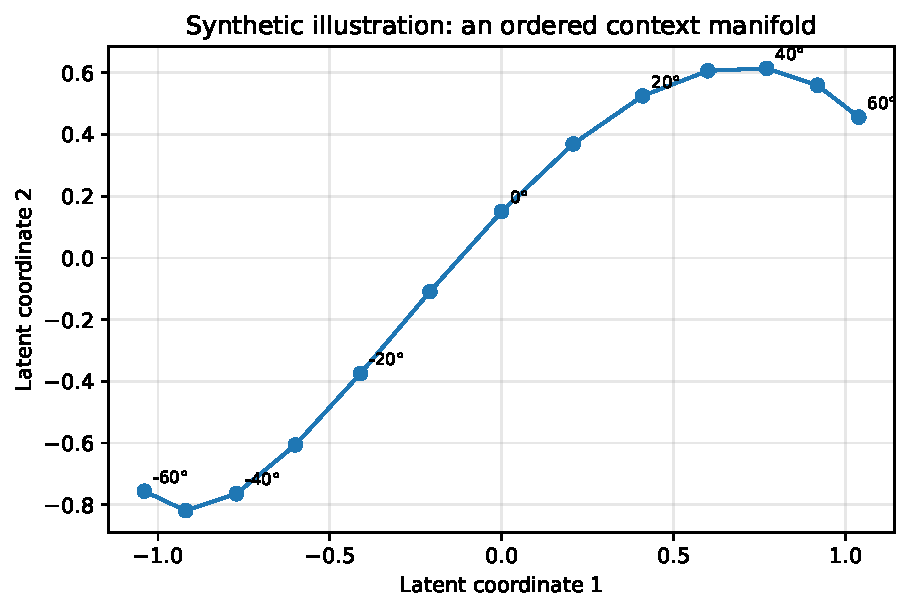
\includegraphics[width=0.72\textwidth]{figures/conceptual_manifold.pdf}
\caption{Synthetic illustration only. A valid descriptive result would show ordered context points with quantitative neighborhood preservation and null-model comparisons.}
\label{fig:toy-manifold}
\end{figure}

\begin{figure}[H]
\centering
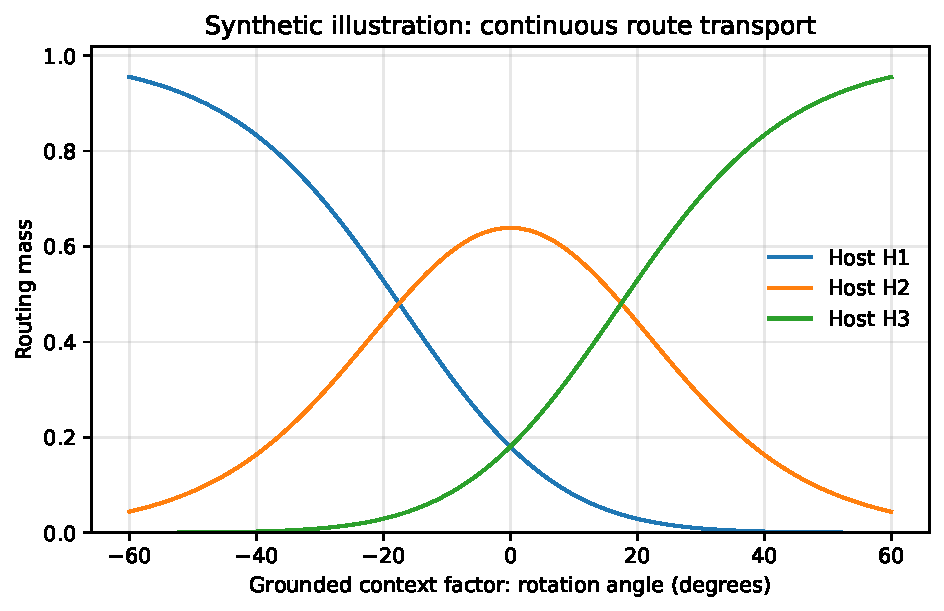
\includegraphics[width=0.72\textwidth]{figures/route_trajectory.pdf}
\caption{Synthetic illustration only. Routing may vary smoothly across context while multiple hosts overlap near transition regions. Smoothness without contribution evidence is not specialization.}
\label{fig:toy-route}
\end{figure}

\begin{figure}[H]
\centering
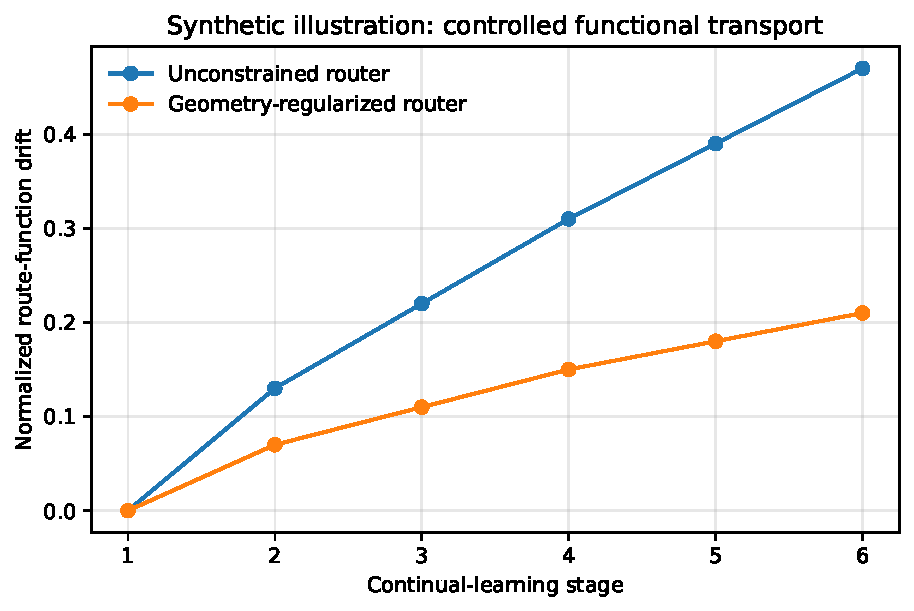
\includegraphics[width=0.72\textwidth]{figures/transport_drift.pdf}
\caption{Synthetic illustration only. The G1 operational hypothesis is that a geometric constraint reduces destructive route-function drift at matched predictive performance and resource budget.}
\label{fig:toy-drift}
\end{figure}

\section{Losses and training policy}

\subsection{Composite G1 loss}

A first practical loss is

\begin{equation}
\begin{split}
\loss_{\mathrm{G1}}=
&\loss_{\mathrm{CE}}
+\lambda_{\mathrm{distill}}\loss_{\mathrm{distill}}
+\lambda_{\mathrm{route}}\loss_{\mathrm{route\text{-}geo}}
+\lambda_{\mathrm{stress}}\loss_{\mathrm{stress}}\\
&+\lambda_{\mathrm{far}}\loss_{\mathrm{far}}
+\lambda_{\mathrm{transport}}\loss_{\mathrm{transport}}
+\lambda_{\mathrm{div}}\loss_{\mathrm{host\text{-}div}}
+\lambda_C C_{\mathrm{carbon}}.
\end{split}
\end{equation}

The host-diversity term should be contribution-aware. A naive penalty that merely pushes representations apart can manufacture useless differentiation. One option is

\begin{equation}
\loss_{\mathrm{host\text{-}div}}=
\sum_{h<k}\underbrace{\bar r_h\bar r_k}_{\text{co-activation}}
\max\bigl(0,m_F-d_F(h,k)\bigr)^2,
\end{equation}

applied only when both hosts are active and the local task loss indicates room for complementary improvement.

\subsection{Transport constraint}

For replay anchors \(A\), the route-function transport loss is

\begin{equation}
\loss_{\mathrm{transport}}=
\E_{x\in A}\left[
\alpha_R d_{\mathrm{FR}}(r_t(x),r_{t-1}(x))^2
+\alpha_Z\norm{z_{M,t}(x)-Qz_{M,t-1}(x)}^2
+\alpha_P\KL(p_{t-1}\|p_t)
\right].
\end{equation}

This is a functional preservation rule, not a requirement to freeze all representations. The alignment \(Q\) permits benign coordinate drift.

\subsection{Avoiding collapse and artificial fragmentation}

Two opposing failures are possible.

\paragraph{Collapse.} One host receives nearly all route mass; host outputs become nearly identical; context inference loses discriminative structure.

\paragraph{Artificial fragmentation.} Every context receives a separate host despite shared structure; compute and memory grow; transfer falls.

The desired regime is a hub-and-partners ecology: one or more broadly useful hosts may act as hubs, while other hosts provide repeatable local gains. A 25/25 unique-host partition is not automatically better than 6--7 meaningful specialists.

\section{Evaluation metrics and acceptance gates}

\subsection{Metric families}

\begin{longtable}{@{}p{3.3cm}p{5.2cm}p{6.3cm}@{}}
\caption{Core G1 metrics.}\label{tab:metrics}\\
\toprule
\textbf{Family} & \textbf{Metric} & \textbf{Interpretation} \\
\midrule
\endfirsthead
\toprule
\textbf{Family} & \textbf{Metric} & \textbf{Interpretation} \\
\midrule
\endhead
Predictive & accuracy, NLL, ECE, Brier score & Current performance and calibration. \\
Continual & final average accuracy, forgetting, intransigence & Retention and plasticity; positive backward transfer is measured but not claimed unless demonstrated. \\
Grounded geometry & Spearman \(\rho\), stress, neighborhood preservation & Alignment with known context factor. \\
Route geometry & Fisher-Rao drift, JS drift, entropy, top-\(k\) occupancy & Smoothness, uncertainty, and collapse. \\
Host specialization & contribution gain, ablation map, CKA, functional distance & Distinctive and useful host roles. \\
Causal & tangent slope, CSR, identity preservation & Specific functional effect of geometric interventions. \\
Transport & Procrustes drift, OT distance, prototype/covariance drift & Controlled deformation of learned structure. \\
Reproducibility & matched-role correlation, seed variance, bootstrap CI & Whether geometry and specialization recur. \\
Efficiency & active FLOPs, latency, route entropy, memory bytes & Carbon-cost proxy. \\
Audit & reconstruction fidelity, trace completeness & Ability to explain and replay route-function behavior. \\
\bottomrule
\end{longtable}

\subsection{Pre-registered gates}

The following pilot thresholds are intentionally conservative and must be frozen before a qualification run. They are not universal constants; they are a preregistration scaffold that prevents post-hoc threshold selection.

\begin{enumerate}[label=\textbf{Gate \arabic*:}]
\item \textbf{Grounding.} The 95\% bootstrap confidence interval lower bound for \(\rho_R\), \(\rho_C\), or \(\rho_{z_M}\) exceeds the 95th percentile of a shuffled-factor null and the point estimate is at least \(0.25\). Neighborhood preservation must exceed a matched-dimensional random control by at least \(0.10\). Normalized stress must be below \(0.70\) or improve the frozen \(z_0\) reference by at least \(10\%\).
\item \textbf{Interpolation.} On held-out intermediate angles, full G1 must beat nearest-trained-context and unconstrained-router controls. Performance on trained angles may drop by at most two accuracy points relative to the unconstrained MMALS variant, unless a preregistered cost or retention objective explicitly permits the trade-off.
\item \textbf{Causality.} Tangent interventions must produce monotonic angle-consistent route changes. The causal specificity ratio must satisfy \(\mathrm{CSR}>1.5\), with a bootstrap 95\% confidence interval lower bound above \(1.0\). Orthogonal controls are matched by norm, and class-identity degradation must remain below the declared margin, by default \(0.05\) nats of target log-probability or one accuracy point.
\item \textbf{Specialization.} At least two non-redundant host roles must show positive local contribution gain, ablation locality ratio at least \(1.5\), and cross-seed role similarity at least \(0.50\) linear CKA after Hungarian matching. A hub-and-partners ecology is admissible; raw dominance is not.
\item \textbf{Transport.} Old-region Procrustes or OT drift must be at least \(10\%\) lower than the softmax baseline, and forgetting must not be worse by more than \(0.5\) accuracy point at matched compute and memory.
\item \textbf{Robustness.} Pilot evidence requires at least five seeds; final qualification requires at least ten seeds. Failed seeds remain in the report and cannot be silently discarded.
\end{enumerate}

A model can pass some gates and fail others. Results must be reported as a profile, not compressed into a single celebratory score.

\section{Experimental phases beyond RotatedMNIST}

\subsection{G1-A: controlled geometry}

\begin{itemize}
\item Continuous RotatedMNIST.
\item Rotated FashionMNIST to test more complex class boundaries.
\item Optional translation, scale, blur, and contrast factors, one at a time before mixing them.
\end{itemize}

\subsection{G1-B: mixed factors and local charts}

Real context may not fit one global coordinate. Introduce two-factor streams such as rotation plus corruption. The model may require local charts \(\{(U_\alpha,\varphi_\alpha)\}\) rather than a single global embedding. The test is whether transition maps preserve functional neighborhoods.

\subsection{G1-C: mature sensory grove on natural images}

Use Split-CIFAR10 first, then Split-CIFAR100. A raw flattened RGB MLP is not an adequate sensory geometry; a pretrained or jointly validated convolutional encoder is required. The backbone remains frozen in the first natural-image test to isolate MMALS contribution.

Baseline sweeps must include EWC, SI if present, LwF, replay memory size, PNN sanity checks, Sparse-MoE, and a joint upper bound. Best validation-selected baselines are reported rather than arbitrary defaults.

\subsection{G1-D: domain and streaming benchmarks}

Proceed to CORe50 and DomainNetMini, then a mixed continual regime. These benchmarks test whether the geometry survives background, acquisition, viewpoint, and domain shifts that lack a single known scalar factor. At this stage, geometry is grounded through augmentations, temporal continuity, metadata, and intervention tests rather than angle alone.

\section{Implementation blueprint}

\subsection{Module interfaces}

A minimal implementation exposes the following tensors for every batch:

\begin{lstlisting}[language=Python]
trace = {
    "z0": sensory_features,          # [B, d0]
    "context": context_embedding,   # [B, dc]
    "route": route_weights,         # [B, H]
    "host_outputs": host_outputs,   # [B, H, dM]
    "z_mmalls": synthesis,          # [B, dM]
    "logits": logits,               # [B, C]
    "memory_ids": memory_ids,
    "cost": active_compute_proxy,
}
\end{lstlisting}

The router, host, and memory APIs must remain independent enough to support ablation.

\subsection{Training pseudocode}

\begin{lstlisting}[language=Python]
for stage, train_loader in continual_stream:
    for batch in train_loader:
        x, y, u_eval = batch  # u_eval is withheld from inference
        with torch.no_grad():
            z0 = sensory_grove(x)

        context = context_encoder(z0, memory.read_context())
        route = router(z0, context, memory.summary(), goal)
        host_outputs = hosts(z0, context, memory)
        z_mmalls = aggregate(route, host_outputs)
        logits = classifier(z_mmalls)

        loss = task_loss(logits, y)
        loss += geometry_losses(context, route, u_eval)
        loss += transport_losses(anchor_batch, model, previous_snapshot)
        loss += specialization_regularizer(route, host_outputs)
        loss += carbon_cost(route, host_outputs, memory)

        optimizer.zero_grad()
        loss.backward()
        optimizer.step()

    evaluate_all_seen_unseen_angles()
    export_route_function_traces()
    memory.compile_and_link_evidence()
\end{lstlisting}

During final task-free experiments, \(u_{\mathrm{eval}}\) is never used in the loss. In controlled G1-A it may be used by a declared geometric regularizer because the purpose is to test whether grounded geometry can be induced and exploited. A second variant removes \(u\) from training to test discovery.

\subsection{Trace schema}

Each trace row contains:

\begin{lstlisting}
dataset, seed, stage, sample_id, true_label, context_factor,
context_vector, route_vector, active_hosts, route_entropy,
host_output_norms, prediction, confidence, loss,
retention_proxy, forgetting_proxy, stability, drift,
compute_cost, memory_cost, contribution_estimates, snapshot_id
\end{lstlisting}

Vectors may be stored in Parquet or NPZ with a relational index. CSV templates are included for lightweight interoperability.

\subsection{Reproducibility contract}

Every final run must record:

\begin{itemize}
\item git commit and environment lock;
\item dataset version and transformation code;
\item seeds for data, initialization, and augmentation;
\item selected hyperparameters and validation criterion;
\item parameter count, active parameters, FLOPs, memory budget, and wall time;
\item all failed runs and exceptions, not only successful outcomes;
\item raw per-seed metrics before aggregation;
\item a claim manifest mapping every statement to an artifact.
\end{itemize}

\section{Failure modes and falsification}

\subsection{Backbone-only geometry}

If \(z_0\) already predicts angle and MMALS adds no interpolation, causal specificity, or operational gain, the correct conclusion is that the sensory grove contains the useful geometry and the MMALS geometry hypothesis is unsupported in that configuration.

\subsection{Projection illusion}

If PCA or UMAP looks ordered but pairwise metrics, held-out interpolation, and null-model tests fail, there is no grounded geometric evidence.

\subsection{Route smoothness without function}

A router can be forced to vary smoothly while hosts remain redundant. This fails the contribution and ablation gates.

\subsection{Specialization by collapse}

A host may dominate because optimization is imbalanced rather than because it is a useful hub. Load balancing, equal initialization, host swapping, and ablation are required to distinguish functional dominance from collapse.

\subsection{Geometry-induced rigidity}

Excessive transport constraints can preserve old geometry while preventing learning. G1 must report both forgetting and intransigence. A lower drift score is not a success if accuracy on new contexts collapses.

\subsection{Unstable host identity}

If apparent host roles change arbitrarily across seeds and cannot be matched by function, the architecture has not demonstrated reproducible specialization.

\subsection{Metric overfitting}

A model may optimize the chosen distance metric without improving behavior. Therefore no single geometry metric is a primary endpoint; descriptive, predictive, causal, and operational tests must agree.

\begin{warningbox}
The G1 hypothesis is falsified for a configuration if the internal geometry does not exceed backbone and shuffled nulls, does not interpolate unseen contexts, does not support specific interventions, or does not improve a concrete objective under matched budgets. A negative result is scientifically useful: it prevents the later energy and phase-aware layers from being built on an empty metaphor.
\end{warningbox}

\section{Relationship to established research}

\subsection{Manifold learning and latent geometry}

Classical manifold learning reconstructs low-dimensional organization from local or global distances \citep{tenenbaum2000isomap,roweis2000lle}. Deep latent geometry extends this by deriving metrics from nonlinear decoders and model sensitivity \citep{arvanitidis2018latent,shao2018riemannian}. Geometry-MMALS differs by treating routes and host functions as first-class geometric objects in a continual, resource-aware system.

\subsection{Mixture of experts}

Sparse MoE systems select a subset of experts per input and can increase capacity without proportional active compute \citep{shazeer2017moe,fedus2022switch}. Patch-level routing also has theoretical sample-efficiency results under specific assumptions \citep{chowdhury2023patchmoe}. G1 does not claim that MMALS is categorically different from MoE. Its proposed distinction is the explicit route-function memory, continual transport, ecological contribution tests, and external audit layer.

\subsection{Continual learning}

Continual learning addresses stability-plasticity and catastrophic forgetting \citep{parisi2019continual,kirkpatrick2017ewc}. Geometric perspectives already appear in parameter-importance walks and task-organized dynamics \citep{chaudhry2018riemannian,duncker2020dynamics}. G1 focuses on observable movement of representations, routes, and host functions, using parameter regularization only as one baseline.

\subsection{Representation comparison and intervention}

CKA provides a robust representation-similarity tool across seeds and architectures \citep{kornblith2019cka}; RTD probes multiscale topology \citep{barannikov2022rtd}; TCAV illustrates how human-meaningful directions can be tested inside networks \citep{kim2018tcav}. G1 combines these with grounded context factors and causal tangent interventions.

\section{Transition to G2 and G3}

\subsection{G2: energy-guided manifold routing}

Only after G1 passes should MMALS define an energy over context, route, memory, and goal:

\begin{equation}
 E_\theta(z,m,c,r;g)=
 \lambda_{\mathrm{fit}}E_{\mathrm{fit}}
 +\lambda_{\mathrm{ret}}E_{\mathrm{ret}}
 +\lambda_C C_{\mathrm{carbon}}
 -\lambda_P G_{\mathrm{phosphorus}}
 +\lambda_{\mathrm{geo}}E_{\mathrm{geo}}.
\end{equation}

Routing may then be

\begin{equation}
 r^*=\arg\min_{r\in\simplex}E_\theta(z,m,c,r;g),
\end{equation}

or sampled from a Gibbs distribution. G1 supplies the metric and transport structure that make such an energy meaningful rather than arbitrary.

\subsection{G3: phase-aware or quantum-inspired routing}

A later phase-aware model may assign complex amplitudes to verified route trajectories. The magnitude could derive from G2 energy, while phase represents compatibility among route-function paths. However, without a validated G1 geometry there is no principled definition of neighboring paths, recombination, or coherent transport. Therefore G3 remains explicitly out of scope.

\begin{equation}
\boxed{\text{G1 geometry is a prerequisite, not a cosmetic preface, for G2 energy and G3 interference.}}
\end{equation}

\section{Claim discipline and publication strategy}

\subsection{Admissible claims by maturity level}

\begin{table}[H]
\centering
\caption{Claim ladder for Geometry-MMALS.}
\label{tab:claims}
\begin{tabularx}{\textwidth}{@{}p{1.2cm}p{4cm}Y@{}}
\toprule
\textbf{Code} & \textbf{Claim} & \textbf{Minimum evidence} \\
\midrule
C0 & Pipeline validity & Reproducible smoke test, no result claim. \\
C1 & External audit/control geometry & Trace vector construction and objective-conditioned selection. \\
C2 & Grounded internal order & L1 descriptive gate on controlled factor. \\
C3 & Predictive manifold & Held-out interpolation and extrapolation gains. \\
C4 & Causal functional geometry & Specific tangent interventions with controls. \\
C5 & Operational Geometry-MMALS & Better retention/stability/cost/specialization at matched budgets. \\
C6 & Cross-benchmark robustness & Repeated effects on natural-image and domain streams. \\
C7 & Energy-guided geometric control & G2 energy improves control beyond G1. \\
C8 & Phase-aware benefit & G3 outperforms real-valued alternatives; no quantum advantage claim without quantum hardware evidence. \\
\bottomrule
\end{tabularx}
\end{table}

The first paper should target C2--C5 on controlled benchmarks. It should not combine every future layer into one universal claim.

\subsection{What the paper must say about negative evidence}

A credible report includes collapsed routes, failed seeds, sensitivity to backbone choice, hyperparameter dependence, and cases where the geometric regularizer harms plasticity. MMALS currently has evidence aligned with retention, forgetting reduction, auditability, and regime-conditioned deployment; positive backward transfer should be measured but not claimed unless the new experiments establish it.

\section{Conclusion}

Geometry-MMALS G1 turns a broad intuition into a falsifiable engineering program. It separates external audit geometry from internal functional geometry; distinguishes sensory, context, route, host, synthesis, and memory spaces; defines metrics appropriate to each space; and requires geometry to pass descriptive, predictive, causal, and operational tests. It also places host specialization on a stronger foundation: not as route frequency, but as reproducible local contribution to the complete MMALS ecosystem.

The first decisive experiment is deliberately simple. A frozen sensory grove processes continuously rotated digits. MMALS must infer the context, route across hosts, interpolate unseen angles, preserve route-function structure through sequential learning, and respond coherently to latent tangent interventions. If it cannot do this, more elaborate geometric or quantum-inspired language should stop. If it can, G1 provides the missing foundation for energy-guided routing, goal-adaptive control, and later phase-aware research.

\begin{plainbox}
The practical promise is a continual learner that does not merely remember outputs. It remembers how regions of experience relate, which transformations are useful there, how those transformations cooperate, how the structure changes over time, and when a new situation lies safely between known ones or outside the system's competence.
\end{plainbox}

\section*{Repository contents}

The companion repository includes:

\begin{itemize}
\item this LaTeX source and compiled PDF;
\item a Colab-ready notebook scaffold;
\item PyTorch modules for the G1 model, geometry losses, and metrics;
\item YAML configuration for RotatedMNIST;
\item trace and result schemas;
\item claim gates and experiment protocol;
\item figure-generation scripts and synthetic smoke tests;
\item a citation file and reproducibility checklist.
\end{itemize}

\section*{Acknowledgment of status}

This article formalizes an evolving independent research program. It is intentionally explicit about the boundary between existing MMALS evidence, proposed mechanisms, synthetic illustrations, and future hypotheses. The purpose is to make the next experiment implementable and criticizable before stronger claims are attempted.

\bibliographystyle{plainnat}
\bibliography{references}

\appendix

\section{TPUT--G1 notation bridge}

MMALS-TPUT and Geometry-MMALS G1 describe two levels of the same stack. TPUT specifies operational policy selection and deployment control; G1 asks whether the internal representation-route-host-memory system has a grounded functional geometry. The symbols should therefore be read with the following bridge.

\begin{longtable}{@{}p{2.6cm}p{3.4cm}p{4.0cm}p{4.2cm}@{}}
\toprule
\textbf{Layer} & \textbf{TPUT object} & \textbf{G1 object} & \textbf{Role} \\
\midrule
Input representation & \(z\) & \(z_0=P(x)\) & Frozen or controlled sensory representation. \\
Context & inferred context state & \(c=q_\phi(z_0)\) & Learned coordinate or local chart. \\
Route & route/action distribution & \(r\in\Delta^{H-1}\) & Host access on the simplex. \\
Host function & host/action module & \(g_h(z_0)\) & Functional transformation field. \\
Synthesis & selected output state & \(z_M=\sum_h r_h g_h(z_0)\) & MMALS synthesized representation. \\
Memory & \(m=(m_{rec},m_{syn})\) & reconstructive plus synthetic memory & Trace replay and compiled reuse. \\
Objective & goal vector \(g\) & goal weights & Experiment or deployment goal. \\
Audit & trace/evidence vector & \(a(x,t)\) & External control geometry, not proof of internal geometry. \\
\bottomrule
\end{longtable}

TPUT may write a deployment energy as
\begin{equation}
E_\theta(r;z,m,g)=E_{fit}+E_{mem}+E_{ret}+E_{cost}+E_{drift}+E_{spec}+E_{audit}.
\end{equation}
G1 may write a training and evidence objective as
\begin{equation}
\loss_{G1}=\loss_{CE}+\lambda_d\loss_{distill}+\lambda_r\loss_{route-geo}+\lambda_s\loss_{stress}+\lambda_f\loss_{far}+\lambda_t\loss_{transport}+\lambda_h\loss_{host-div}+\lambda_c C_{carbon}.
\end{equation}
These are not contradictory. The TPUT form is the policy-control view; the G1 form is the experimental proof view. The bridge is: fit corresponds to task loss and calibration; memory to reconstructive fidelity and compiled reuse; retention to forgetting and old-region transport; cost to active FLOPs and carbon proxies; drift to geometric and Hydro diagnostics; specialization to contribution, ablation and CKA evidence; audit to trace completeness and reconstructive memory.

\section{Suggested result tables}

\begin{table}[H]
\centering
\caption{Primary performance and continual-learning table template.}
\begin{tabularx}{\textwidth}{@{}Y C C C C C@{}}
\toprule
Model & Final avg. acc. & Forgetting & NLL & Active FLOPs & Memory MB \\
\midrule
Backbone + linear & -- & -- & -- & -- & -- \\
Sparse MoE & -- & -- & -- & -- & -- \\
MMALS softmax & -- & -- & -- & -- & -- \\
MMALS route-geo & -- & -- & -- & -- & -- \\
MMALS full G1 & -- & -- & -- & -- & -- \\
Joint upper bound & -- & n/a & -- & -- & -- \\
\bottomrule
\end{tabularx}
\end{table}

\begin{table}[H]
\centering
\caption{Geometry evidence table template.}
\begin{tabularx}{\textwidth}{@{}Y C C C C C@{}}
\toprule
Layer & \(\rho\) angle-distance & Stress & kNN preservation & Interp. error & CSR \\
\midrule
Sensory \(z_0\) & -- & -- & -- & -- & -- \\
Context \(c\) & -- & -- & -- & -- & -- \\
Route \(r\) & -- & -- & -- & -- & -- \\
Synthesis \(z_M\) & -- & -- & -- & -- & -- \\
\bottomrule
\end{tabularx}
\end{table}

\begin{table}[H]
\centering
\caption{Host specialization table template.}
\begin{tabularx}{\textwidth}{@{}Y C C C C C@{}}
\toprule
Host role & Peak context & Contribution gain & Ablation locality & Mean CKA to peers & Cross-seed match \\
\midrule
H1 / matched role A & -- & -- & -- & -- & -- \\
H2 / matched role B & -- & -- & -- & -- & -- \\
H3 / matched role C & -- & -- & -- & -- & -- \\
\bottomrule
\end{tabularx}
\end{table}

\section{Suggested ablation matrix}

\begin{longtable}{@{}p{4cm}p{5cm}p{5cm}@{}}
\toprule
\textbf{Ablation} & \textbf{Question} & \textbf{Expected diagnostic} \\
\midrule
Remove route geometry & Does simplex continuity matter? & Higher interpolation error or route drift. \\
Remove far-pair contrast & Is smoothness collapsing routes? & Lower route diversity and weaker contribution maps. \\
Remove transport loss & Does geometric memory preserve old regions? & Higher drift and forgetting. \\
Remove host diversity term & Are hosts functionally redundant? & Higher CKA and lower ablation locality. \\
Freeze hosts & Is routing alone sufficient? & Reveals value of adaptive host transformations. \\
Uniform route & Is learned access necessary? & Measures benefit of specialization. \\
Oracle angle & What is the context-inference ceiling? & Diagnostic upper bound, not deployable result. \\
Unfreeze sensory grove & Does end-to-end adaptation improve or confound geometry? & Compare backbone and MMALS contributions. \\
Replace Fisher-Rao with Euclidean & Is simplex-aware geometry useful? & Metric-specific sensitivity. \\
Remove reconstructive memory & Is audit trace needed for recovery and debugging? & Lower reconstruction fidelity. \\
Remove synthetic memory & Is compiled reuse reducing cost? & Higher latency and memory recomputation. \\
\bottomrule
\end{longtable}

\section{Minimal claim manifest schema}

\begin{lstlisting}
claim_id: C4_tangent_intervention
statement: "The learned context direction for rotation has a specific causal effect on routing."
status: proposed | supported | failed
primary_metric: causal_specificity_ratio
acceptance_gate: bootstrap_CI_lower > 1.0 and identity_drop < margin
artifacts:
  - results/per_seed/causal_intervention.csv
  - figures/causal_tangent_controls.pdf
  - logs/run_manifest.json
limitations:
  - controlled RotatedMNIST only
  - no claim of general causal representation learning
\end{lstlisting}

\end{document}
